\documentclass[15pt]{article}
\usepackage[utf8]{inputenc}
\usepackage{natbib}
\usepackage{graphicx}
\usepackage{float}
\usepackage{array}
\usepackage{tabularx}
\usepackage{geometry}
\usepackage{titlesec}
\usepackage{sectsty}
\usepackage{enumitem}
\usepackage{lipsum}
\usepackage{longtable}
\usepackage{booktabs,xltabular}
\usepackage{setspace}
\usepackage{tocloft,lipsum,pgffor,sectsty}
\usepackage{tocbasic}
\usepackage[font=Large,labelfont=bf]{caption}
\usepackage{enumitem}
\usepackage[toc,page]{appendix}
\usepackage{hyperref}
\usepackage{colortbl}
\hypersetup{
    colorlinks=true,
    linkcolor=black,
    filecolor=black,      
    urlcolor=blue,
    anchorcolor = black,
    citecolor=black
}

 \geometry{
 a4paper,
 total={170mm,257mm},
 left=20mm,
 top=20mm,
 }

\titleformat*{\section}{\LARGE\bfseries}
\titleformat*{\subsection}{\tiny\bfseries}
\titleformat*{\subsubsection}{\large\bfseries}
\titleformat*{\paragraph}{\large\bfseries}
\titleformat*{\subparagraph}{\large\bfseries}

\begin{document}

\begin{titlepage}

\addtolength{\hoffset}{-0.1cm}
	\centering
	
\includegraphics[width=0.60\textwidth]{logo.png}\par\vspace{1.5cm}
	{\huge\bfseries SOEN 6481 \par}
	{\huge\bfseries Software Systems Requirements Specification \par}
	{\scshape\LARGE Fall 2019 \par}
	\vspace{1cm}
	\vspace{1.5cm}
	{\huge\bfseries Ticket Vending Machine \par}
	{\huge\bfseries Requirements Specification \par}
	\vspace{1cm}
	{\scshape\LARGE Team F - Deliverable 2\par}

	\vspace{0.5cm}
	\begin{tabular}{ c l }
	\vspace{0.2cm}
	{\Large\bfseries 40083289 \par} & {\Large Dhaval Chandreshkumar Modi \par}\\
	\vspace{0.2cm}
	{\Large\bfseries 40084358 \par} & {\Large Dolly Modha  \par}\\
	\vspace{0.2cm}
	{\Large\bfseries 40085480 \par} & {\Large Liangzhao Lin  \par}\\
	\vspace{0.2cm}
	{\Large\bfseries 40082567 \par} & {\Large Naren Morabagal Somasekhar \par}\\
	\vspace{0.2cm}
	{\Large\bfseries 40076735 \par} & {\Large Pruthvi Raju Nallaparaju \par}\\
	\end{tabular}
	\vspace{0.5cm}

    \vspace{0.5cm}

	\vfill

	\vspace{0.2cm}
	{\large Supervised By} \par
    \vspace{0.2cm}
	{\Large Prof. Pankaj Kamthan}

	\vfill
	{\Large Google Drive : \url{http://bit.ly/2ON5C1C}\par}
	\vspace{0.2cm}
    {\Large Github Repo: \url{http://bit.ly/2IQRBMt}}

	\vfill

% Bottom of the page
	{\large \today\par}
	\par
    
\end{titlepage}


\renewcommand{\cftpartfont}{\Large\bfseries}
\renewcommand\cftsecfont{\Large\bfseries}
\renewcommand\cftsecpagefont{\Large\bfseries}
\renewcommand{\cftsubsecfont}{\Large\bfseries}
\renewcommand{\cftsubsecpagefont}{\Large\bfseries}
\renewcommand\cftsecafterpnum{\par\addvspace{6pt}}
\renewcommand\cftloftitlefont{\Large\bfseries}
\renewcommand\cftfigfont{\Large\bfseries}
\renewcommand\cftfigpagefont{\Large\bfseries}




\doublespacing
\tableofcontents
\singlespacing
\setlength{\cftparskip}{1\baselineskip}
\listoffigures

\subsectionfont{\Large}



\newpage
\section{\Large{User Story}}
\Large{In software development and product management, a user story is an informal, natural language description of one or more features of a software system. \cite{cohn2004user}
}
\subsection{\Large{User Story Format}}


\begin{figure}[H]
\centering
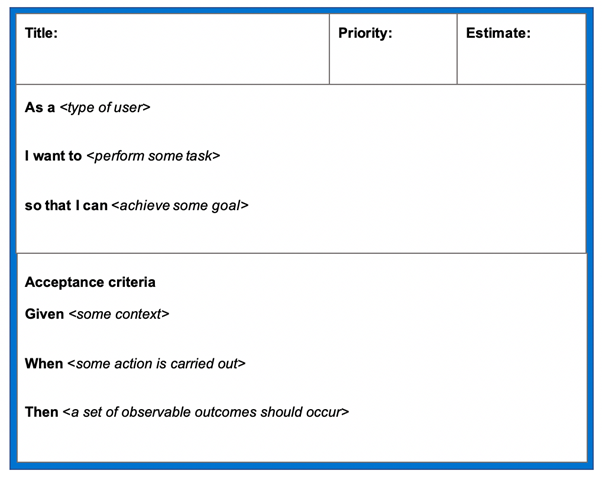
\includegraphics[width=0.60\textwidth]{User_Story_Format.png}\par\vspace{0.1cm}
\caption{\Large\bfseries{User Story Format}}
\label{User Story Format:do}
\end{figure}

\Large{This is the template of our user story for TVM.
}

\subsection{\Large{Priority Scale}}
\Large{This scale is defined considering the functionality, scope and how critical it is to the system during the further stages of software engineering.\cite{popli2014prioritising} 
}

\begin{longtable}{| p{.18\textwidth} | p{.18\textwidth} | p{.18\textwidth} | p{.18\textwidth} | p{.18\textwidth} |} 
 \hline
  {\bfseries Very Low} & {\bfseries Low} & {\bfseries Moderate} & {\bfseries High} & {\bfseries Very High} \\
 \hline
  \end{longtable}

\subsection{\Large{Story Point Estimate Scale}}
\Large{A story point is a metric used in agile project management and development to estimate the difficulty of implementing a given user story, which is an abstract measure of effort required to implement it. In simple terms, a story point is a number that tells the difficulty level of the story.\cite{coelho2012effort} {\bfseries The scale is 1, 2, 3, 5, 8.}
}

\section{Personas\cite{sim2014empowering}}
\subsection{Persona : Student}
\vspace{0.5cm}

\begin{figure}[H]
\centering
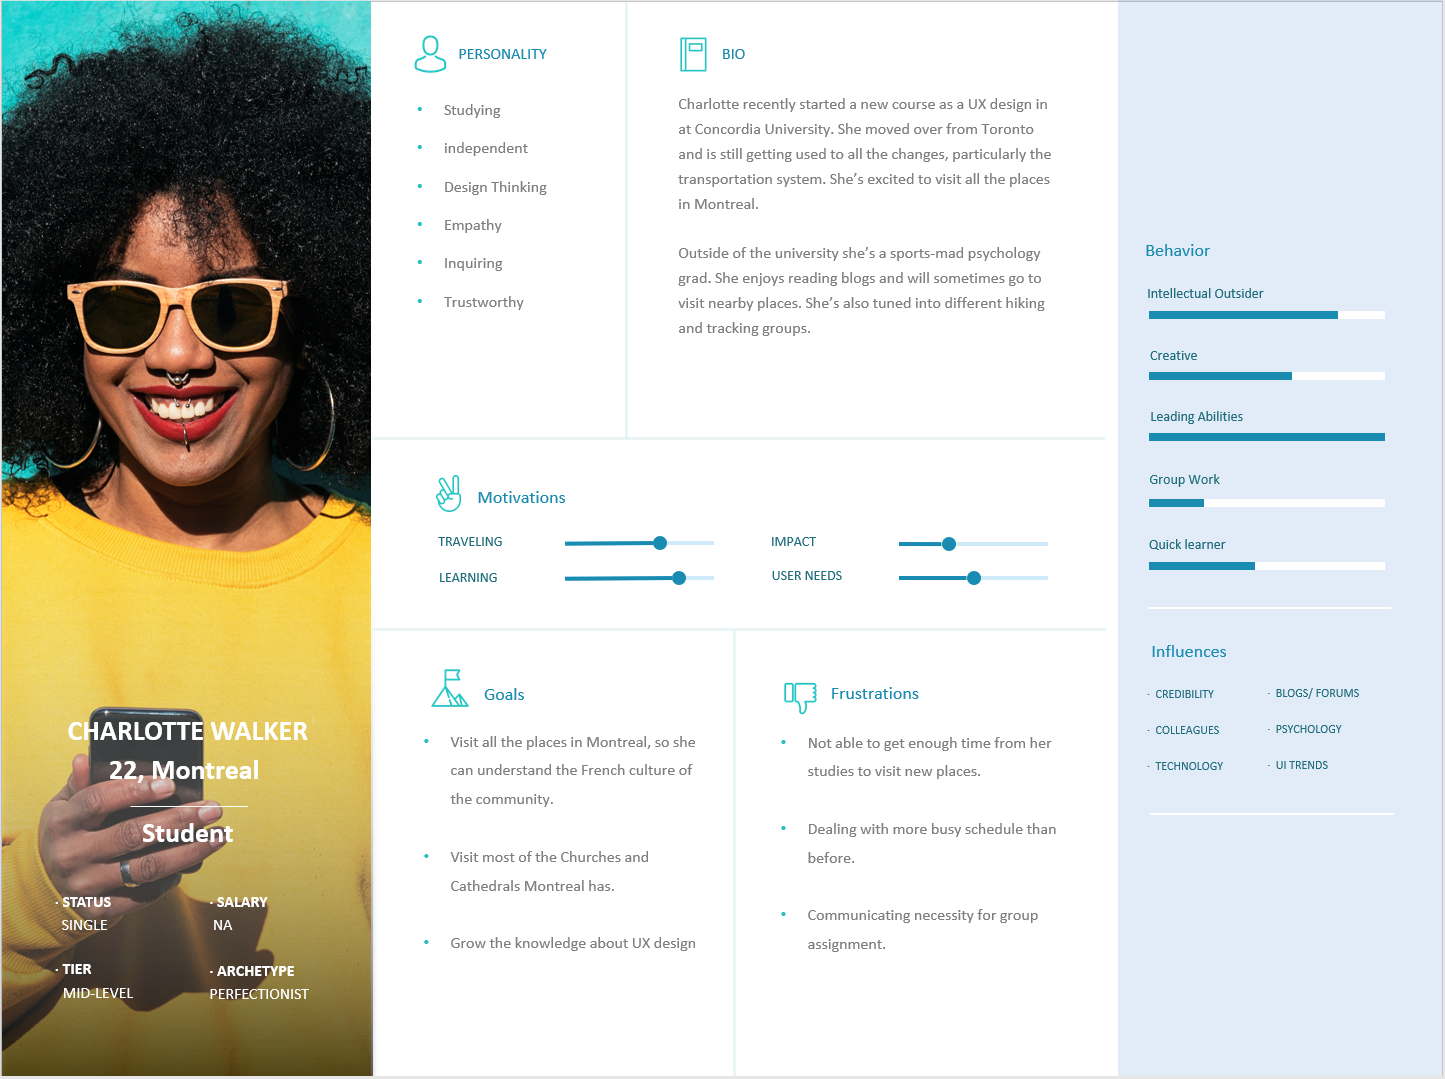
\includegraphics[width=1\textwidth]{Persona1.PNG}\par\vspace{0.1cm}
\caption{\Large\bfseries{Persona : Student}}
\label{Persona : Student:do}
\end{figure}

This persona represents archetypes NOT stereotypes of a broader student segment or group. A student persona summarizes who the student users are and why they are using the TVM, as well as what behaviors, assumptions, and expectations determine their view of the TVM.
\subsection{Persona : Senior Citizen}
\vspace{0.5cm}

\begin{figure}[H]
\centering
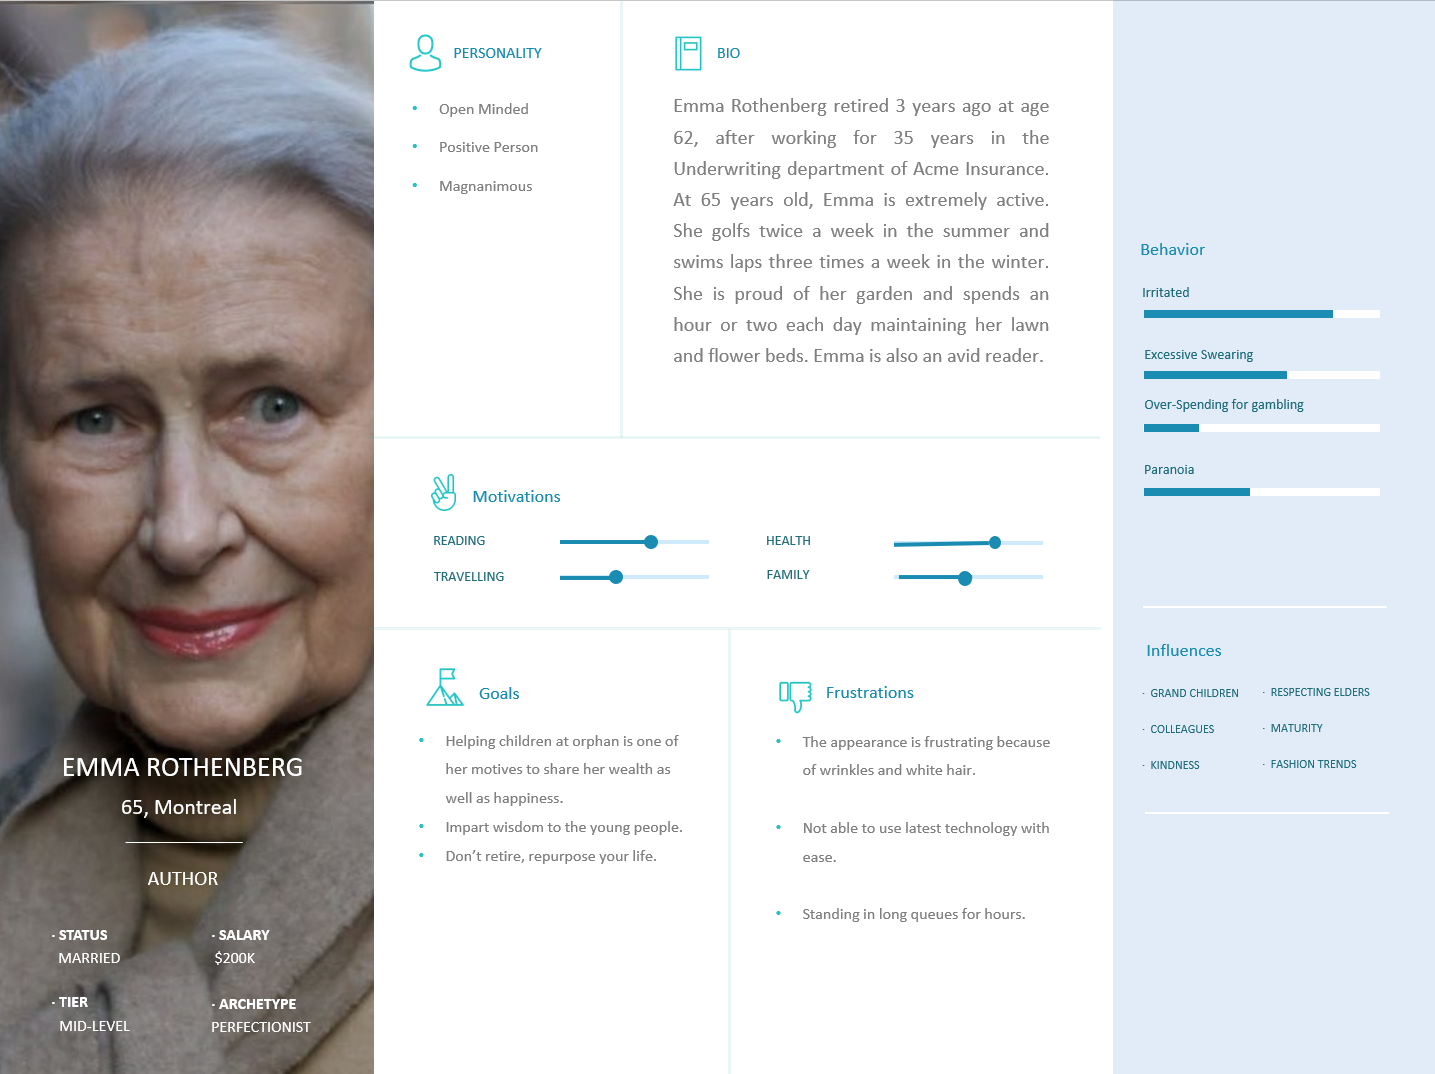
\includegraphics[width=1\textwidth]{Persona2.PNG}\par\vspace{0.1cm}
\caption{\Large\bfseries{Persona : Senior Citizen}}
\label{Persona : Senior Citizen:do}
\end{figure}


This persona represents archetypes NOT stereotypes of a broader Senior Citizen segment or group. A senior citizen persona summarizes who the old age users are and why they are using the TVM, as well as what behaviors, assumptions, and expectations determine their view of the TVM.
\subsection{Persona : Hacker}
\vspace{0.5cm}

\begin{figure}[H]
\centering
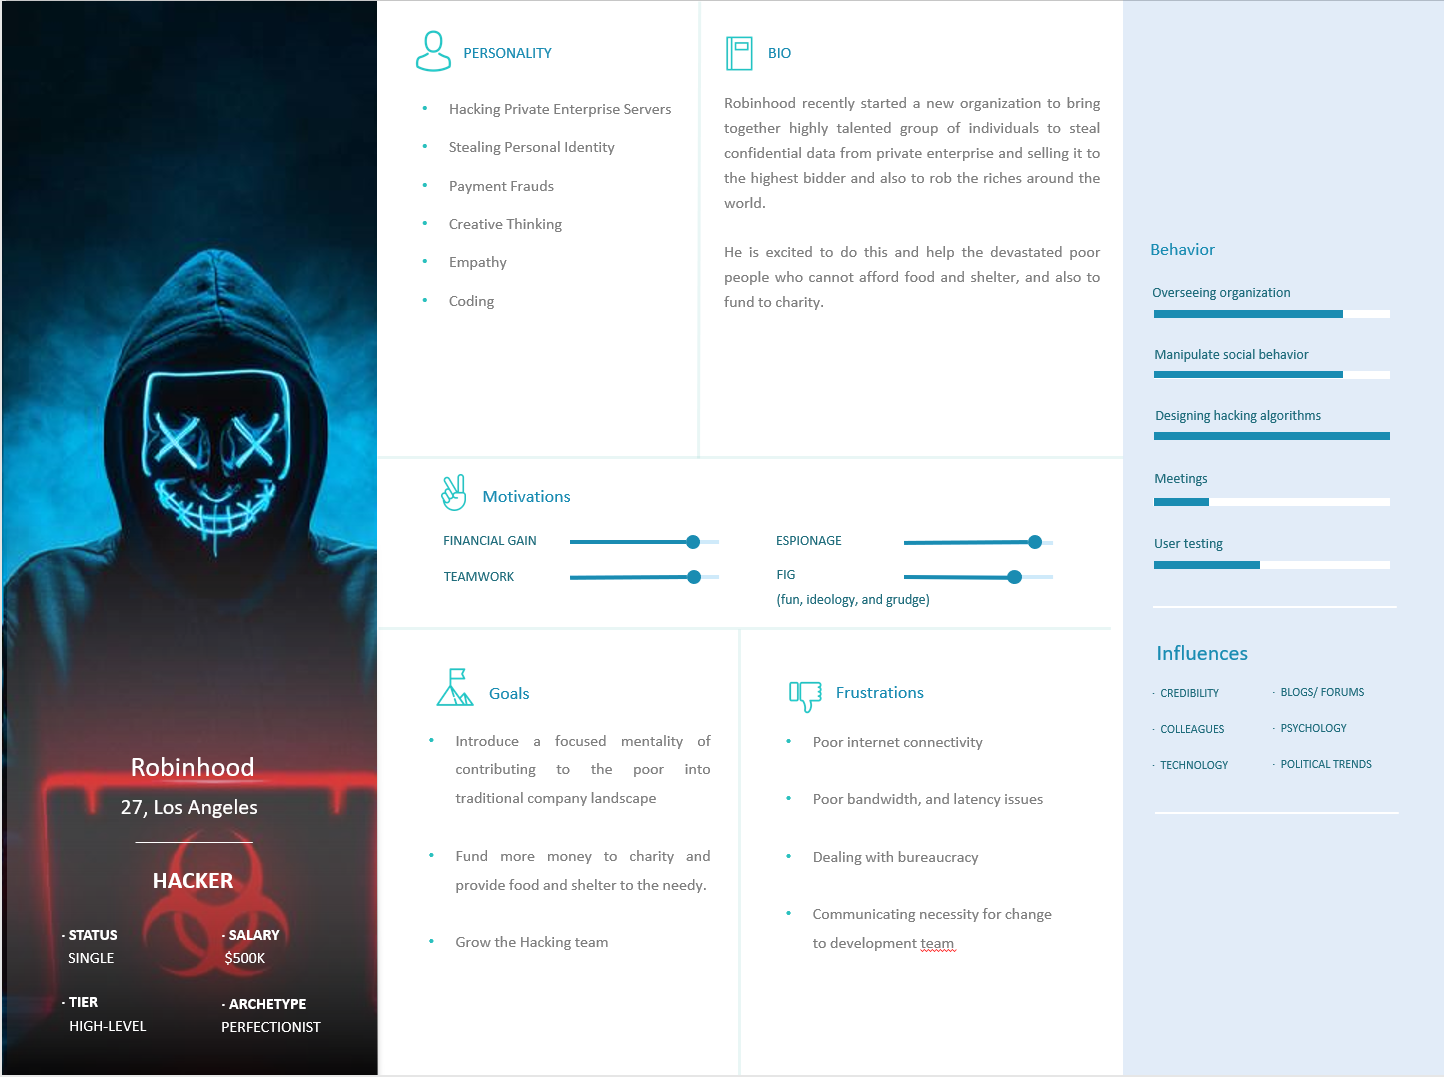
\includegraphics[width=1\textwidth]{Persona3.PNG}\par\vspace{0.1cm}
\caption{\Large\bfseries{Persona : Hacker}}
\label{Persona : Hacker:do}
\end{figure}

This persona represents archetypes NOT stereotypes of a broader hacker segment or group. A hacker persona summarizes who the hacker users are and why they are using the TVM, as well as what behaviors, assumptions, and expectations determine their view of the TVM.


\newpage
\section{\Large{User Stories}}

\subsection{\Large{Constraints}}
\begin{itemize}
    \item {\bfseries Support Sustainability and Productivity : } By tracing our user stories backwards to Use case model, Domain model, Activity Diagram, and Sequence diagram we are able to remove redundant and invalid user stories and test cases which reduces the overall time and cost of implementation of the system and to test them. \cite{calero2013towards}
    \item {\bfseries Support Re-usability : } Implementation of user stories such as payment by cash or card can be reused with many other implementation which uses similar mode of payment with very less modification. Also, implementation of user stories such select preferred language and select type of ticket etc,. can be reused to build Ticket Vending Machine for some other geological location. \cite{adams2015nonfunctional}
\end{itemize}

\newpage
\subsection{\Large{List of User Stories}}

  \bgroup
\def\arraystretch{2}
\begin{longtable}{!{\color{black}\vrule width 5pt} p{.4\textwidth} !{\color{black}\vrule width 1pt} p{.3\textwidth} !{\color{black}\vrule width 1pt} p{.2\textwidth} !{\color{black}\vrule width 5pt}} 
   \noalign{\global\arrayrulewidth=2mm}
  \arrayrulecolor{black}\hline
  
  

{\bfseries Title : Selection of Language (US01)} & {\bfseries Priority : Moderate} & {\bfseries Estimate : 1 }\\ [0.5ex] 
  \noalign{\global\arrayrulewidth=0.5mm}
  \arrayrulecolor{black}\hline
  \multicolumn{3}{!{\color{black}\vrule width 5pt} p{.9\textwidth} !{\color{black}\vrule width 5pt}}{{\bfseries As}  a commuter I want to select the language (English/French) from the user interface of ticket vending machine.
  
  {\bfseries I want to} choose a language(English/ French).
  
  {\bfseries So that I can} read the instructions/options in familiar language, on the ticket vending machine interface.
} \\
 \noalign{\global\arrayrulewidth=0.5mm}
  \arrayrulecolor{black}\hline
\multicolumn{3}{!{\color{black}\vrule width 5pt} p{.9\textwidth} !{\color{black}\vrule width 5pt}}{
  \vspace{5pt}
  {\bfseries Constraints }
  \newline
  {\bfseries Support Policy : } read the instructions/options in familiar language, on the ticket vending machine interface.
  \newline
   {\bfseries Support Verifiability : } If the commuter select any of the language, TVM user interface should display instructions in selected language only.
}
\\

\hline
\multicolumn{3}{!{\color{black}\vrule width 5pt} p{.9\textwidth} !{\color{black}\vrule width 5pt}}{
  \vspace{5pt}
  {\bfseries Acceptance Test }
  
  {\bfseries Given } that a commuter wants to purchase a ticket but he/she is only familiar with one of the languages. Several reasons such as 1. He/She is an international student and only knows English language, then he/she chooses English language  2. He/She is a native and only knows french language, then he/she chooses french language.
  \newline
   {\bfseries When } the language is chosen, TVM shows further instructions in chosen language.
   \newline
   {\bfseries Then } 2 things happen, 1. Displays different options of tickets  2. Takes them back to the home page(or main page).
   \newline
   {\bfseries Result } Test Pass.
} \\

\hline
\multicolumn{3}{!{\color{black}\vrule width 5pt} p{.9\textwidth} !{\color{black}\vrule width 5pt}}{
  {\bfseries Formulated By :} Dhaval Modi
} \\

\hline
\multicolumn{3}{!{\color{black}\vrule width 5pt} p{.9\textwidth} !{\color{black}\vrule width 5pt}}{
  {\bfseries Implemented By :}
} \\
  \noalign{\global\arrayrulewidth=2mm}
  \arrayrulecolor{black}\hline

  \end{longtable}
  
  
 
 
 
 
 
 
 
 
 
 \newpage
 \begin{longtable}{!{\color{black}\vrule width 5pt} p{.4\textwidth} !{\color{black}\vrule width 1pt} p{.3\textwidth} !{\color{black}\vrule width 1pt} p{.2\textwidth} !{\color{black}\vrule width 5pt}} 
   \noalign{\global\arrayrulewidth=2mm}
  \arrayrulecolor{black}\hline
  
  

{\bfseries Title : Selection of Ticket (US02)} & {\bfseries Priority : High} & {\bfseries Estimate : 2 }\\ [0.5ex] 
  \noalign{\global\arrayrulewidth=0.5mm}
  \arrayrulecolor{black}\hline
  \multicolumn{3}{!{\color{black}\vrule width 5pt} p{.9\textwidth} !{\color{black}\vrule width 5pt}}{{\bfseries As} a commuter who wants to choose the type of ticket (one way / two way / weekly pass / monthly pass) from the user interface of ticket vending machine.
  
  {\bfseries I want to}  choose a type of ticket.
  
  {\bfseries So that I can} I can pay for the ticket and commute.

} \\
 \noalign{\global\arrayrulewidth=0.5mm}
  \arrayrulecolor{black}\hline
\multicolumn{3}{!{\color{black}\vrule width 5pt} p{.9\textwidth} !{\color{black}\vrule width 5pt}}{
  \vspace{5pt}
  {\bfseries Constraints }
  \newline
  {\bfseries Support Decidability: } The user can make a decision about which type of ticket he/she wants to buy, for example, one way, two way, weekly pass or monthly pass. The user can also decide to continue to buy a ticket or change their mind to recharge their card.
  
}
\\

\hline
\multicolumn{3}{!{\color{black}\vrule width 5pt} p{.9\textwidth} !{\color{black}\vrule width 5pt}}{
  \vspace{5pt}
  {\bfseries Acceptance Test }
  
  {\bfseries Given } that a commuter wants to purchase a type of ticket but he/she has many options. Several reasons such as 1. He/She wants to travel for one way, he/she might choose one way ticket option 2. He/She wants to travel somewhere and to come back home, so he/she might prefer two way ticket option. 3. Commuter is only in the city for a week, he/she might take prefer weekly pass 4. For budgetary reasons, he/she might prefer monthly pass.
  \newline
   {\bfseries When } I choose any of the ticket options, the TVM proceeds with the chosen type of ticket.
   \newline
   {\bfseries Then } 2 things happen, 1. Displays different options of payment methods 2. Takes them back to the home page(or main page).
   \newline
   {\bfseries Result } Test Pass.
} \\

\hline
\multicolumn{3}{!{\color{black}\vrule width 5pt} p{.9\textwidth} !{\color{black}\vrule width 5pt}}{
  {\bfseries Formulated By :} Dhaval Modi
} \\

\hline
\multicolumn{3}{!{\color{black}\vrule width 5pt} p{.9\textwidth} !{\color{black}\vrule width 5pt}}{
  {\bfseries Implemented By :}
} \\
  \noalign{\global\arrayrulewidth=2mm}
  \arrayrulecolor{black}\hline

  \end{longtable}
  
  
  
  
  
  
  
  
  
  
  
  
  
  
  
  
  
  \newpage
  \begin{longtable}{!{\color{black}\vrule width 5pt} p{.4\textwidth} !{\color{black}\vrule width 1pt} p{.3\textwidth} !{\color{black}\vrule width 1pt} p{.2\textwidth} !{\color{black}\vrule width 5pt}} 
   \noalign{\global\arrayrulewidth=2mm}
  \arrayrulecolor{black}\hline
  
  

{\bfseries Title : Recharge Travel Card(US03)} & {\bfseries Priority : Moderate} & {\bfseries Estimate : 5 }\\ [0.5ex] 
  \noalign{\global\arrayrulewidth=0.5mm}
  \arrayrulecolor{black}\hline
  \multicolumn{3}{!{\color{black}\vrule width 5pt} p{.9\textwidth} !{\color{black}\vrule width 5pt}}{{\bfseries As} a commuter I want to recharge my travel card because I use public transport frequently.
  
  {\bfseries I want to} recharge my travel card.
  
  {\bfseries So that I can}  use public transport facilities. 
} \\
 \noalign{\global\arrayrulewidth=0.5mm}
  \arrayrulecolor{black}\hline
\multicolumn{3}{!{\color{black}\vrule width 5pt} p{.9\textwidth} !{\color{black}\vrule width 5pt}}{
  \vspace{5pt}
  {\bfseries Constraints }
  \newline
  {\bfseries Support Clarity : } There is minimal or no ambiguity in this process. The user has clarity that recharging the card will recharge the card and terminate the process.
  \newline
   {\bfseries Support Validatability : }  It validates the travel card. For example, it will display a message when recharge is successful which validates that the card is recharged and can be used for the next commute.
}
\\

\hline
\multicolumn{3}{!{\color{black}\vrule width 5pt} p{.9\textwidth} !{\color{black}\vrule width 5pt}}{
  \vspace{5pt}
  {\bfseries Acceptance Test }
  
  {\bfseries Given }  that a commuter wants to recharger his/her travel card, they chose the option “Recharge Card”
  \newline
   {\bfseries When } recharge card is selected it, the system asks the commuter to insert the travel card and will take the user through the payment process.
   \newline
   {\bfseries Then }  on the success of payment process, the card is successfully recharged and can be used for the commute.
   \newline
   {\bfseries Result } Test Pass.
} \\

\hline
\multicolumn{3}{!{\color{black}\vrule width 5pt} p{.9\textwidth} !{\color{black}\vrule width 5pt}}{
  {\bfseries Formulated By :} Dolly Modha
} \\

\hline
\multicolumn{3}{!{\color{black}\vrule width 5pt} p{.9\textwidth} !{\color{black}\vrule width 5pt}}{
  {\bfseries Implemented By :} Naren Morabagal Somasekhar
} \\
  \noalign{\global\arrayrulewidth=2mm}
  \arrayrulecolor{black}\hline

  \end{longtable}
  
  
  
  
  
  
  
  
  
  
  
  
  
  
  
  
  
  
  
  \newpage
  \begin{longtable}{!{\color{black}\vrule width 5pt} p{.4\textwidth} !{\color{black}\vrule width 1pt} p{.3\textwidth} !{\color{black}\vrule width 1pt} p{.2\textwidth} !{\color{black}\vrule width 5pt}} 
   \noalign{\global\arrayrulewidth=2mm}
  \arrayrulecolor{black}\hline
  
  

{\bfseries Title : Select Payment Mode(US04)} & {\bfseries Priority : Moderate} & {\bfseries Estimate : 2 }\\ [0.5ex] 
  \noalign{\global\arrayrulewidth=0.5mm}
  \arrayrulecolor{black}\hline
  \multicolumn{3}{!{\color{black}\vrule width 5pt} p{.9\textwidth} !{\color{black}\vrule width 5pt}}{{\bfseries As}  commuter I want to pay for my purchase of a ticket or recharging the card.
  
  {\bfseries I want to} select the payment mode and proceed to pay in chosen method.
  
  {\bfseries So that I can}  complete my payment in the selected mode.
} \\
 \noalign{\global\arrayrulewidth=0.5mm}
  \arrayrulecolor{black}\hline
\multicolumn{3}{!{\color{black}\vrule width 5pt} p{.9\textwidth} !{\color{black}\vrule width 5pt}}{
  \vspace{5pt}
  {\bfseries Constraints }
  \newline
  {\bfseries Support Clarity : }  There minimal or no ambiguity in this process. The user has clarity about the mode of payment i.e., he/she wants to either pay by cash or pay by card.
  \newline
   {\bfseries Support Decidability : }  User can make a decision about which payment mode they want to select and continue with either by card or by cash.
}
\\

\hline
\multicolumn{3}{!{\color{black}\vrule width 5pt} p{.9\textwidth} !{\color{black}\vrule width 5pt}}{
  \vspace{5pt}
  {\bfseries Acceptance Test }
  
  {\bfseries Given } that the commuter has 2 options for modes of payment either by card (debit/credit) or by cash.
  \newline
   {\bfseries When } Commuter selects the mode of payment i.e,. either by card or by cash.
   \newline
   {\bfseries Then } Commuter confirms the payment mode and continues to make the payment in preferred mode.
   \newline
   {\bfseries Result } Test Pass.
} \\

\hline
\multicolumn{3}{!{\color{black}\vrule width 5pt} p{.9\textwidth} !{\color{black}\vrule width 5pt}}{
  {\bfseries Formulated By :} Dolly Modha
} \\

\hline
\multicolumn{3}{!{\color{black}\vrule width 5pt} p{.9\textwidth} !{\color{black}\vrule width 5pt}}{
  {\bfseries Implemented By :} Dhaval Modi
} \\
  \noalign{\global\arrayrulewidth=2mm}
  \arrayrulecolor{black}\hline

  \end{longtable}
  
  
  
  
  
  
  
  
  
  
  
  
  
  
  
  
  
  
  
  
  
  
  
  \newpage
  \begin{longtable}{!{\color{black}\vrule width 5pt} p{.4\textwidth} !{\color{black}\vrule width 1pt} p{.3\textwidth} !{\color{black}\vrule width 1pt} p{.2\textwidth} !{\color{black}\vrule width 5pt}} 
   \noalign{\global\arrayrulewidth=2mm}
  \arrayrulecolor{black}\hline
  
  

{\bfseries Title : Payment by cash(US05)} & {\bfseries Priority : High} & {\bfseries Estimate : 5 }\\ [0.5ex] 
  \noalign{\global\arrayrulewidth=0.5mm}
  \arrayrulecolor{black}\hline
  \multicolumn{3}{!{\color{black}\vrule width 5pt} p{.9\textwidth} !{\color{black}\vrule width 5pt}}{{\bfseries As} Commuter selects to pay by cash.
  
  {\bfseries I want to} use cash to pay my transaction.
  
  {\bfseries So that I can} complete my transaction then get payment receipt (and ticket).
} \\
 \noalign{\global\arrayrulewidth=0.5mm}
  \arrayrulecolor{black}\hline
\multicolumn{3}{!{\color{black}\vrule width 5pt} p{.9\textwidth} !{\color{black}\vrule width 5pt}}{
  \vspace{5pt}
  {\bfseries Constraints }
  \newline
  {\bfseries Support Policy : } The TVM accepts Canadian cash only in the following denominations: 
  \newline - 0.25\$, 0.5\$, 1\$, 2\$ coins 
  \newline - 5\$, 10\$, 20\$, 50\$, 100\$ bills
}
\\

\hline
\multicolumn{3}{!{\color{black}\vrule width 5pt} p{.9\textwidth} !{\color{black}\vrule width 5pt}}{
  \vspace{5pt}
  {\bfseries Acceptance Test }
  
  {\bfseries Given } payment by cash.
  \newline
   {\bfseries When } the amount of cash inserted equal to or greater than the amount to be paid.
   \newline
   {\bfseries Then } the transaction is paid and completed, receipt (and ticket)  are printed and   refund is returned.
   \newline
   {\bfseries Result } Test Pass.
} \\

\hline
\multicolumn{3}{!{\color{black}\vrule width 5pt} p{.9\textwidth} !{\color{black}\vrule width 5pt}}{
  {\bfseries Formulated By :} Liangzhao Lin
} \\

\hline
\multicolumn{3}{!{\color{black}\vrule width 5pt} p{.9\textwidth} !{\color{black}\vrule width 5pt}}{
  {\bfseries Implemented By :}
} \\
  \noalign{\global\arrayrulewidth=2mm}
  \arrayrulecolor{black}\hline

  \end{longtable}
  
  
  
  
  
  
  
  
  
  
  
  
  
  
  
  
  \newpage
  \begin{longtable}{!{\color{black}\vrule width 5pt} p{.4\textwidth} !{\color{black}\vrule width 1pt} p{.3\textwidth} !{\color{black}\vrule width 1pt} p{.2\textwidth} !{\color{black}\vrule width 5pt}} 
   \noalign{\global\arrayrulewidth=2mm}
  \arrayrulecolor{black}\hline
  
  

{\bfseries Title : Payment by card(US06)} & {\bfseries Priority : High} & {\bfseries Estimate : 8 }\\ [0.5ex] 
  \noalign{\global\arrayrulewidth=0.5mm}
  \arrayrulecolor{black}\hline
  \multicolumn{3}{!{\color{black}\vrule width 5pt} p{.9\textwidth} !{\color{black}\vrule width 5pt}}{{\bfseries As} commuter I select to pay by card.
  
  {\bfseries I want to} insert my credit/debit card and pay my transaction by card.
  
  {\bfseries So that I can}  complete my transaction then get payment receipt (and ticket).
} \\
 \noalign{\global\arrayrulewidth=0.5mm}
  \arrayrulecolor{black}\hline
\multicolumn{3}{!{\color{black}\vrule width 5pt} p{.9\textwidth} !{\color{black}\vrule width 5pt}}{
  \vspace{5pt}
  {\bfseries Constraints }
  \newline
  {\bfseries Security specific : } There should be connection and validation of the card between TVM and bank in order to process the transaction.
  \newline
   {\bfseries Support Policy : }  The credit/debit card should have sufficient credit/balance in the selected account to pay the amount.
}
\\

\hline
\multicolumn{3}{!{\color{black}\vrule width 5pt} p{.9\textwidth} !{\color{black}\vrule width 5pt}}{
  \vspace{5pt}
  {\bfseries Acceptance Test }
  
  {\bfseries Given } payment by card.
  \newline
   {\bfseries When } 
   \newline 1.The credit/debit card inserted is valid.
   \newline 2.The card (credit/debit) PIN entered is valid.
   \newline 3.The payment transaction is validated, approved by the Bank and received by the
  TVM.
   \newline
   {\bfseries Then } the transaction is paid and completed, receipt (and ticket)  are printed.
   \newline
   {\bfseries Result } Test Pass.
} \\

\hline
\multicolumn{3}{!{\color{black}\vrule width 5pt} p{.9\textwidth} !{\color{black}\vrule width 5pt}}{
  {\bfseries Formulated By :} Liangzhao Lin
} \\

\hline
\multicolumn{3}{!{\color{black}\vrule width 5pt} p{.9\textwidth} !{\color{black}\vrule width 5pt}}{
  {\bfseries Implemented By :} Dolly Modha
} \\
  \noalign{\global\arrayrulewidth=2mm}
  \arrayrulecolor{black}\hline

  \end{longtable}
  
  
  
  
  
  
  
  
  
  
  
  
  
  
  
  
  
  
  
  
  
  \newpage
  \begin{longtable}{!{\color{black}\vrule width 5pt} p{.4\textwidth} !{\color{black}\vrule width 1pt} p{.3\textwidth} !{\color{black}\vrule width 1pt} p{.2\textwidth} !{\color{black}\vrule width 5pt}} 
   \noalign{\global\arrayrulewidth=2mm}
  \arrayrulecolor{black}\hline
  
  

{\bfseries Title : Cancellation of Transaction(US07)} & {\bfseries Priority : High} & {\bfseries Estimate : 5 }\\ [0.5ex] 
  \noalign{\global\arrayrulewidth=0.5mm}
  \arrayrulecolor{black}\hline
  \multicolumn{3}{!{\color{black}\vrule width 5pt} p{.9\textwidth} !{\color{black}\vrule width 5pt}}{{\bfseries As}  commuter I want to cancel the transaction of a ticket purchase or recharge the travel card.
  
  {\bfseries I want to} cancel an active transaction.
  
  {\bfseries So that I can} start another transaction because I decided to buy a different type of ticket or make a different mode of payment. Or maybe I just move away from the TVM because I changed my mind and don’t want to use the transport service.
} \\
 \noalign{\global\arrayrulewidth=0.5mm}
  \arrayrulecolor{black}\hline
\multicolumn{3}{!{\color{black}\vrule width 5pt} p{.9\textwidth} !{\color{black}\vrule width 5pt}}{
  \vspace{5pt}
  {\bfseries Constraints }
  \newline
  {\bfseries Support Clarity : } There is minimal or no ambiguity in this process. The user has clarity that pressing the button cancel will cancel the transaction and terminate the process.
  \newline
   {\bfseries Support Decidability : }  The user can make a decision of purchasing a ticket or making payment. For example, the user can decide to continue with the transaction or decide to cancel it by clicking the cancel button.
}
\\

\hline
\multicolumn{3}{!{\color{black}\vrule width 5pt} p{.9\textwidth} !{\color{black}\vrule width 5pt}}{
  \vspace{5pt}
  {\bfseries Acceptance Test }
  
  {\bfseries Given } that a commuter is purchasing a ticket or recharging the card, or making a payment, he/she can decide to cancel the transaction due to several reasons such as 1. to buy a different type, 2. make a different mode of payment 3. Not wanting to purchase the ticket anymore, they can ‘hit’ the option ‘cancel’.
  \newline
   {\bfseries When } the option ‘cancel’ is selected, the TVM aborts the ongoing active transaction.
   \newline
   {\bfseries Then } 2 things happen, 1. Displays a ‘Transaction Cancelled’ message to the user of TVM and 2. Takes them back to the home page(or main page).
   \newline
   {\bfseries Result } Test Pass.
} \\

\hline
\multicolumn{3}{!{\color{black}\vrule width 5pt} p{.9\textwidth} !{\color{black}\vrule width 5pt}}{
  {\bfseries Formulated By :} Naren Morabagal Somasekhar
} \\

\hline
\multicolumn{3}{!{\color{black}\vrule width 5pt} p{.9\textwidth} !{\color{black}\vrule width 5pt}}{
  {\bfseries Implemented By :} Liangzhao Lin
} \\
  \noalign{\global\arrayrulewidth=2mm}
  \arrayrulecolor{black}\hline

  \end{longtable}
  
  
  
  
  
  
  
  
  
  
  
  
  
  
  
  
  \newpage
  \begin{longtable}{!{\color{black}\vrule width 5pt} p{.4\textwidth} !{\color{black}\vrule width 1pt} p{.3\textwidth} !{\color{black}\vrule width 1pt} p{.2\textwidth} !{\color{black}\vrule width 5pt}} 
   \noalign{\global\arrayrulewidth=2mm}
  \arrayrulecolor{black}\hline
  
  

{\bfseries Title :  Purchase a ticket(US08)} & {\bfseries Priority : Very High} & {\bfseries Estimate : 8 }\\ [0.5ex] 
  \noalign{\global\arrayrulewidth=0.5mm}
  \arrayrulecolor{black}\hline
  \multicolumn{3}{!{\color{black}\vrule width 5pt} p{.9\textwidth} !{\color{black}\vrule width 5pt}}{{\bfseries As} a commuter I would like to select the type of ticket.
  
  {\bfseries I want to} select the ticket from the available options.
  
  {\bfseries So that I can} access the metro for travelling.
} \\
 \noalign{\global\arrayrulewidth=0.5mm}
  \arrayrulecolor{black}\hline
\multicolumn{3}{!{\color{black}\vrule width 5pt} p{.9\textwidth} !{\color{black}\vrule width 5pt}}{
  \vspace{5pt}
  {\bfseries Constraints }
  \newline
  {\bfseries Usability specific : } Commuter who purchases a ticket will not get a refund if he/she wants to purchase another ticket instead.
  \newline
   {\bfseries Security specific : } TVM should be able to check for fake currency notes or coins.
}
\\

\hline
\multicolumn{3}{!{\color{black}\vrule width 5pt} p{.9\textwidth} !{\color{black}\vrule width 5pt}}{
  \vspace{5pt}
  {\bfseries Acceptance Test }
  
  {\bfseries Given } Commuter views the available tickets like one-day, one week, etc.
  \newline
   {\bfseries When } Commuter chooses the language and ready for selecting ticket.
   \newline
   {\bfseries Then } Commuter selects the ticket and he/she is ready for payment.
   \newline
   {\bfseries Result } Test Pass.
} \\

\hline
\multicolumn{3}{!{\color{black}\vrule width 5pt} p{.9\textwidth} !{\color{black}\vrule width 5pt}}{
  {\bfseries Formulated By :} Pruthvi Raju Nallaparaju
} \\

\hline
\multicolumn{3}{!{\color{black}\vrule width 5pt} p{.9\textwidth} !{\color{black}\vrule width 5pt}}{
  {\bfseries Implemented By :}
} \\
  \noalign{\global\arrayrulewidth=2mm}
  \arrayrulecolor{black}\hline

  \end{longtable}
  
  
  
  
  
  
  
  
  
  
  
  
  
  
  
  
  
  \newpage
  \begin{longtable}{!{\color{black}\vrule width 5pt} p{.4\textwidth} !{\color{black}\vrule width 1pt} p{.3\textwidth} !{\color{black}\vrule width 1pt} p{.2\textwidth} !{\color{black}\vrule width 5pt}} 
   \noalign{\global\arrayrulewidth=2mm}
  \arrayrulecolor{black}\hline
  
  

{\bfseries Title : Steal Card Information(US09)} & {\bfseries Priority : Very High} & {\bfseries Estimate : 8 }\\ [0.5ex] 
  \noalign{\global\arrayrulewidth=0.5mm}
  \arrayrulecolor{black}\hline
  \multicolumn{3}{!{\color{black}\vrule width 5pt} p{.9\textwidth} !{\color{black}\vrule width 5pt}}{{\bfseries As} a fraud I want to steal the card details of the user.
  
  {\bfseries I want to}  get into the TVM and is in a position to steal the data.
  
  {\bfseries So that I can} uses the data like card details and PIN in order to steal the commuter money.
} \\
 \noalign{\global\arrayrulewidth=0.5mm}
  \arrayrulecolor{black}\hline
\multicolumn{3}{!{\color{black}\vrule width 5pt} p{.9\textwidth} !{\color{black}\vrule width 5pt}}{
  \vspace{5pt}
  {\bfseries Constraints }
  \newline
  {\bfseries Security Specific : } Due to security issues in the TVM, hackers could be able to get the access of the TVM so that he/she can steal the card information and use it for fraudulent transactions.
  \newline
   {\bfseries Support Verifiability : } If the commuter select any of the language, TVM user interface should display instructions in selected language only.
}
\\

\hline
\multicolumn{3}{!{\color{black}\vrule width 5pt} p{.9\textwidth} !{\color{black}\vrule width 5pt}}{
  \vspace{5pt}
  {\bfseries Acceptance Test }
  
  {\bfseries Given } that a hacker hacks the TVM system when a user tries to pay by card.
  \newline
   {\bfseries When } Commuter enters the PIN.
   \newline
   {\bfseries Then } hacker steals the money from commuter bank account.
   \newline
   {\bfseries Result } Test Pass.
} \\

\hline
\multicolumn{3}{!{\color{black}\vrule width 5pt} p{.9\textwidth} !{\color{black}\vrule width 5pt}}{
  {\bfseries Formulated By :} Pruthvi Raju Nallaparaju
} \\

\hline
\multicolumn{3}{!{\color{black}\vrule width 5pt} p{.9\textwidth} !{\color{black}\vrule width 5pt}}{
  {\bfseries Implemented By :}
} \\
  \noalign{\global\arrayrulewidth=2mm}
  \arrayrulecolor{black}\hline

  \end{longtable}
  
  
  
  
  
  
  
  
  
  
  
  
  
  
  
  
  
  
  \newpage
  \begin{longtable}{!{\color{black}\vrule width 5pt} p{.4\textwidth} !{\color{black}\vrule width 1pt} p{.3\textwidth} !{\color{black}\vrule width 1pt} p{.2\textwidth} !{\color{black}\vrule width 5pt}} 
   \noalign{\global\arrayrulewidth=2mm}
  \arrayrulecolor{black}\hline
  
  

{\bfseries Title : Payment Fraud(US10)} & {\bfseries Priority : Very High} & {\bfseries Estimate : 8 }\\ [0.5ex] 
  \noalign{\global\arrayrulewidth=0.5mm}
  \arrayrulecolor{black}\hline
  \multicolumn{3}{!{\color{black}\vrule width 5pt} p{.9\textwidth} !{\color{black}\vrule width 5pt}}{{\bfseries As}  hacker/Fraud or a Bad guy I want to steal money
  
  {\bfseries I want to} breach the TVM security and hack the system.
  
  {\bfseries So that I can}  steal sensitive information such as credit or debit card number and PIN number and steal money.
} \\
 \noalign{\global\arrayrulewidth=0.5mm}
  \arrayrulecolor{black}\hline
\multicolumn{3}{!{\color{black}\vrule width 5pt} p{.9\textwidth} !{\color{black}\vrule width 5pt}}{
  \vspace{5pt}
  {\bfseries Constraints }
  \newline
  {\bfseries Support Policy : }  There may be a loophole in the security of the TVM, because of which the Hacker has an opportunity to penetrate into the system and eventually steal money.
}
\\

\hline
\multicolumn{3}{!{\color{black}\vrule width 5pt} p{.9\textwidth} !{\color{black}\vrule width 5pt}}{
  \vspace{5pt}
  {\bfseries Acceptance Test }
  
  {\bfseries Given } a commuter is purchasing a ticket or recharging the card and making a cashless payment by his/her debit/credit card.
  \newline
   {\bfseries When }  the TVM user inserts their credit/debit card and enters the PIN number.
   \newline
   {\bfseries Then } by sniffing or spoofing the system, sensitive information like card number and PIN number is stolen to make a fraud transaction and steal money.
   \newline
   {\bfseries Result } Test Pass.
} \\

\hline
\multicolumn{3}{!{\color{black}\vrule width 5pt} p{.9\textwidth} !{\color{black}\vrule width 5pt}}{
  {\bfseries Formulated By :} Naren Morabagal Somasekhar
} \\

\hline
\multicolumn{3}{!{\color{black}\vrule width 5pt} p{.9\textwidth} !{\color{black}\vrule width 5pt}}{
  {\bfseries Implemented By :}
} \\
  \noalign{\global\arrayrulewidth=2mm}
  \arrayrulecolor{black}\hline

  \end{longtable}
  

\newpage
\section{\Large Traceability Matrix} Traceability is a commitment to software requirements management.\cite{cleland2012software} It is thereby an
attribute of a software artifact or of a collection of software artifacts.\cite{cleland2014software}
The table below is a backward traceability matrix for TVM user stories.

\begin{center}
\begin{longtable}{| p{.40\textwidth} | p{.60\textwidth} |} 
   \noalign{\global\arrayrulewidth=1mm}
  \arrayrulecolor{black}\hline
  {\bfseries User Story} & {\bfseries Source} \\ [0.5ex] 
 \hline
 Selection of Language (US01) & 
 \begin{itemize}
  \item S1: Use Case Model of TVM and UC01.
  \item S2: Context of Use Model of TVM.
  \item S3: Domain Model of TVM.
  \item S4: Activity Diagram.
  \end{itemize}  \\ 
 \hline
 
Selection of Ticket (US02)
 &  \begin{itemize}
  \item S1: Use Case Model of TVM and UC03.
  \item S2: Domain Model of TVM.
  \item S3: Activity Diagram.
  \item S4: Purchase Ticket's sequence diagram.
  \end{itemize}   \\
 \hline
 
Selection of Ticket (US03)
 &  \begin{itemize}
  \item S1: Use Case Model of TVM and UC04.
  \item S2: Domain Model of TVM.
  \item S3: Activity Diagram.
  \item S4: Purchase Ticket's sequence diagram.
  \item S5: Description of TVM.
  \end{itemize}   \\
 \hline
 
Selection of Ticket (US04)
 &  \begin{itemize}
  \item S1: Use Case Model of TVM and UC05.
  \item S2: Domain Model of TVM.
  \item S3: Activity Diagram.
  \item S4: Payment Sequence Diagram.
  \end{itemize}   \\
 \hline

Selection of Ticket (US05)
 &  \begin{itemize}
  \item S1: Use Case Model of TVM and UC06.
  \item S2: Domain Model of TVM.
  \item S3: Activity Diagram.
  \item S4: Payment Sequence Diagram.
  \end{itemize}   \\
 \hline
 
Selection of Ticket (US06)
 &  \begin{itemize}
  \item S1: Use Case Model of TVM and UC07.
  \item S2: Domain Model of TVM.
  \item S3: Activity Diagram.
  \item S4: Payment Sequence Diagram.
  \end{itemize}   \\
 \hline
 
Selection of Ticket (US07)
 &  \begin{itemize}
  \item S1: Use Case Model of TVM and UC08.
  \item S2: Domain Model of TVM.
  \item S3: Interview Transcript.
  \end{itemize}   \\
 \hline
 
 Selection of Ticket (US08)
 &  \begin{itemize}
  \item S1: Use Case Model of TVM and UC03.
  \item S2: Domain Model of TVM.
  \item S3: Activity Diagram.
  \item S4: Purchase Ticket Sequence Diagram.
  \item S5: Description of TVM.
  \end{itemize}   \\
 \hline
 
 
 Selection of Ticket (US09)
 &  \begin{itemize}
  \item S1: Use Case Model of TVM and UC09.
  \item S2: Domain Model of TVM.
  \end{itemize}   \\
 \hline
 
 
 
Selection of Ticket (US10)
 &  \begin{itemize}
  \item S1: Use Case Model of TVM and UC10.
  \item S2: Domain Model of TVM.
  \end{itemize}   \\
 [1ex] 
 \hline
\end{longtable}
\end{center}
\vspace{1cm}

This table shows how the user stories can be traced back to the source which are Use case model, Domain model, Activity diagram, and Sequence diagram.


\bibliographystyle{plain}
\bibliography{references}
\end{document}
